

\tikzset{every picture/.style={line width=0.75pt}} %set default line width to 0.75pt        

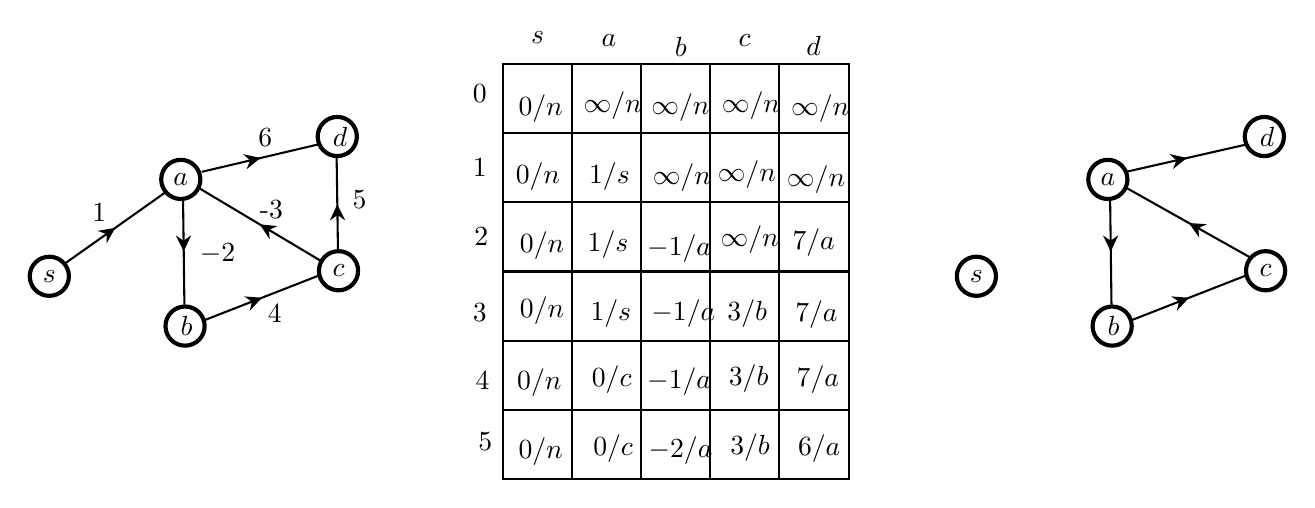
\begin{tikzpicture}[x=0.5pt,y=0.5pt,yscale=-1,xscale=1]
%uncomment if require: \path (0,384); %set diagram left start at 0, and has height of 384

%Shape: Grid [id:dp11668880045661734] 
\draw  [draw opacity=0] (366,45) -- (616,45) -- (616,345) -- (366,345) -- cycle ; \draw   (416,45) -- (416,345)(466,45) -- (466,345)(516,45) -- (516,345)(566,45) -- (566,345) ; \draw   (366,95) -- (616,95)(366,145) -- (616,145)(366,195) -- (616,195)(366,245) -- (616,245)(366,295) -- (616,295) ; \draw   (366,45) -- (616,45) -- (616,345) -- (366,345) -- cycle ;
%Straight Lines [id:da34498379019209924] 
\draw [color={rgb, 255:red, 0; green, 0; blue, 0 }  ,draw opacity=1 ][line width=0.75]    (50,189) -- (122,138) ;
\draw [shift={(86,163.5)}, rotate = 504.69] [fill={rgb, 255:red, 0; green, 0; blue, 0 }  ,fill opacity=1 ][line width=0.08]  [draw opacity=0] (11.61,-5.58) -- (0,0) -- (11.61,5.58) -- (7.71,0) -- cycle    ;
%Straight Lines [id:da15240395104529547] 
\draw [color={rgb, 255:red, 0; green, 0; blue, 0 }  ,draw opacity=1 ][line width=0.75]    (147,135) -- (234,187) ;
\draw [shift={(190.5,161)}, rotate = 30.87] [fill={rgb, 255:red, 0; green, 0; blue, 0 }  ,fill opacity=1 ][line width=0.08]  [draw opacity=0] (11.61,-5.58) -- (0,0) -- (11.61,5.58) -- (7.71,0) -- cycle    ;
%Straight Lines [id:da35482909520855144] 
\draw [color={rgb, 255:red, 0; green, 0; blue, 0 }  ,draw opacity=1 ][line width=0.75]    (233,198) -- (151,230) ;
\draw [shift={(192,214)}, rotate = 158.68] [fill={rgb, 255:red, 0; green, 0; blue, 0 }  ,fill opacity=1 ][line width=0.08]  [draw opacity=0] (11.61,-5.58) -- (0,0) -- (11.61,5.58) -- (7.71,0) -- cycle    ;
%Straight Lines [id:da9934926023449607] 
\draw [color={rgb, 255:red, 0; green, 0; blue, 0 }  ,draw opacity=1 ][line width=0.75]    (135,142) -- (136,219) ;
\draw [shift={(135.5,180.5)}, rotate = 269.26] [fill={rgb, 255:red, 0; green, 0; blue, 0 }  ,fill opacity=1 ][line width=0.08]  [draw opacity=0] (11.61,-5.58) -- (0,0) -- (11.61,5.58) -- (7.71,0) -- cycle    ;
%Straight Lines [id:da7563500509285274] 
\draw [color={rgb, 255:red, 0; green, 0; blue, 0 }  ,draw opacity=1 ][line width=0.75]    (246,112) -- (247,181) ;
\draw [shift={(246.5,146.5)}, rotate = 89.17] [fill={rgb, 255:red, 0; green, 0; blue, 0 }  ,fill opacity=1 ][line width=0.08]  [draw opacity=0] (11.61,-5.58) -- (0,0) -- (11.61,5.58) -- (7.71,0) -- cycle    ;
%Straight Lines [id:da1926158580753592] 
\draw [color={rgb, 255:red, 0; green, 0; blue, 0 }  ,draw opacity=1 ][line width=0.75]    (906.5,185) -- (817.5,135) ;
\draw [shift={(862,160)}, rotate = 389.33000000000004] [fill={rgb, 255:red, 0; green, 0; blue, 0 }  ,fill opacity=1 ][line width=0.08]  [draw opacity=0] (11.61,-5.58) -- (0,0) -- (11.61,5.58) -- (7.71,0) -- cycle    ;
%Straight Lines [id:da5417396008779365] 
\draw [color={rgb, 255:red, 0; green, 0; blue, 0 }  ,draw opacity=1 ][line width=0.75]    (903,198) -- (821,230) ;
\draw [shift={(862,214)}, rotate = 158.68] [fill={rgb, 255:red, 0; green, 0; blue, 0 }  ,fill opacity=1 ][line width=0.08]  [draw opacity=0] (11.61,-5.58) -- (0,0) -- (11.61,5.58) -- (7.71,0) -- cycle    ;
%Straight Lines [id:da8796336265405228] 
\draw [color={rgb, 255:red, 0; green, 0; blue, 0 }  ,draw opacity=1 ][line width=0.75]    (805,142) -- (806,219) ;
\draw [shift={(805.5,180.5)}, rotate = 269.26] [fill={rgb, 255:red, 0; green, 0; blue, 0 }  ,fill opacity=1 ][line width=0.08]  [draw opacity=0] (11.61,-5.58) -- (0,0) -- (11.61,5.58) -- (7.71,0) -- cycle    ;
%Straight Lines [id:da08409930095041618] 
\draw [color={rgb, 255:red, 0; green, 0; blue, 0 }  ,draw opacity=1 ][line width=0.75]    (904.5,103) -- (816.5,123) ;
\draw [shift={(860.5,113)}, rotate = 167.2] [fill={rgb, 255:red, 0; green, 0; blue, 0 }  ,fill opacity=1 ][line width=0.08]  [draw opacity=0] (11.61,-5.58) -- (0,0) -- (11.61,5.58) -- (7.71,0) -- cycle    ;
%Straight Lines [id:da920349957299462] 
\draw [color={rgb, 255:red, 0; green, 0; blue, 0 }  ,draw opacity=1 ][line width=0.75]    (233.5,103) -- (148.5,123) ;
\draw [shift={(191,113)}, rotate = 166.76] [fill={rgb, 255:red, 0; green, 0; blue, 0 }  ,fill opacity=1 ][line width=0.08]  [draw opacity=0] (11.61,-5.58) -- (0,0) -- (11.61,5.58) -- (7.71,0) -- cycle    ;

% Text Node
\draw (375.24,65.06) node [anchor=north west][inner sep=0.75pt]   [align=left] {$\displaystyle 0/n$};
% Text Node
\draw (342.24,111.56) node [anchor=north west][inner sep=0.75pt]   [align=left] {$\displaystyle 1$};
% Text Node
\draw (343.24,161.06) node [anchor=north west][inner sep=0.75pt]   [align=left] {$\displaystyle 2$};
% Text Node
\draw (384.24,19.56) node [anchor=north west][inner sep=0.75pt]   [align=left] {$\displaystyle s$};
% Text Node
\draw (435.24,21.56) node [anchor=north west][inner sep=0.75pt]   [align=left] {$\displaystyle a$};
% Text Node
\draw (488.24,23.56) node [anchor=north west][inner sep=0.75pt]   [align=left] {$\displaystyle b$};
% Text Node
\draw (534.24,21.56) node [anchor=north west][inner sep=0.75pt]   [align=left] {$\displaystyle c$};
% Text Node
\draw (422.24,63.06) node [anchor=north west][inner sep=0.75pt]   [align=left] {$\displaystyle \infty /n$};
% Text Node
\draw (342.24,58.06) node [anchor=north west][inner sep=0.75pt]   [align=left] {$\displaystyle 0$};
% Text Node
\draw (342.24,216.06) node [anchor=north west][inner sep=0.75pt]   [align=left] {$\displaystyle 3$};
% Text Node
\draw (188.24,141.53) node [anchor=north west][inner sep=0.75pt]   [align=left] {\mbox{-}$\displaystyle 3$};
% Text Node
\draw  [line width=1.5]   (38.38, 198.47) circle [x radius= 14.15, y radius= 14.15]   ;
\draw (38.38,198.47) node   [align=left] {$\displaystyle s$};
% Text Node
\draw  [line width=1.5]   (133.38, 128.47) circle [x radius= 14.15, y radius= 14.15]   ;
\draw (133.38,128.47) node   [align=left] {$\displaystyle a$};
% Text Node
\draw  [line width=1.5]   (136.48, 234.47) circle [x radius= 14.15, y radius= 14.15]   ;
\draw (130.98,234.47) node [anchor=west] [inner sep=0.75pt]   [align=left] {$\displaystyle b$};
% Text Node
\draw  [line width=1.5]   (247.38, 194.47) circle [x radius= 14.15, y radius= 14.15]   ;
\draw (247.38,194.47) node   [align=left] {$\displaystyle c$};
% Text Node
\draw (67.24,143.53) node [anchor=north west][inner sep=0.75pt]   [align=left] {$\displaystyle 1$};
% Text Node
\draw (194,217) node [anchor=north west][inner sep=0.75pt]   [align=left] {$\displaystyle 4$};
% Text Node
\draw (145,172.47) node [anchor=north west][inner sep=0.75pt]   [align=left] {$\displaystyle -2$};
% Text Node
\draw (471.24,64.06) node [anchor=north west][inner sep=0.75pt]   [align=left] {$\displaystyle \infty /n$};
% Text Node
\draw (522.24,63.06) node [anchor=north west][inner sep=0.75pt]   [align=left] {$\displaystyle \infty /n$};
% Text Node
\draw (519.24,113.06) node [anchor=north west][inner sep=0.75pt]   [align=left] {$\displaystyle \infty /n$};
% Text Node
\draw (373.24,114.06) node [anchor=north west][inner sep=0.75pt]   [align=left] {$\displaystyle 0/n$};
% Text Node
\draw (376.24,164.06) node [anchor=north west][inner sep=0.75pt]   [align=left] {$\displaystyle 0/n$};
% Text Node
\draw (376.24,211.06) node [anchor=north west][inner sep=0.75pt]   [align=left] {$\displaystyle 0/n$};
% Text Node
\draw (426.24,114.06) node [anchor=north west][inner sep=0.75pt]   [align=left] {$\displaystyle 1/s$};
% Text Node
\draw (472.24,115.06) node [anchor=north west][inner sep=0.75pt]   [align=left] {$\displaystyle \infty /n$};
% Text Node
\draw (521.24,160.06) node [anchor=north west][inner sep=0.75pt]   [align=left] {$\displaystyle \infty /n$};
% Text Node
\draw (425.24,163.06) node [anchor=north west][inner sep=0.75pt]   [align=left] {$\displaystyle 1/s$};
% Text Node
\draw (468.24,166.06) node [anchor=north west][inner sep=0.75pt]   [align=left] {$\displaystyle -1/a$};
% Text Node
\draw (344.24,265.06) node [anchor=north west][inner sep=0.75pt]   [align=left] {$\displaystyle 4$};
% Text Node
\draw (583.24,22.56) node [anchor=north west][inner sep=0.75pt]   [align=left] {$\displaystyle d$};
% Text Node
\draw  [line width=1.5]   (246.48, 97.47) circle [x radius= 14.15, y radius= 14.15]   ;
\draw (240.98,97.47) node [anchor=west] [inner sep=0.75pt]   [align=left] {$\displaystyle d$};
% Text Node
\draw (255.24,134.53) node [anchor=north west][inner sep=0.75pt]   [align=left] {$\displaystyle 5$};
% Text Node
\draw (572.24,65.06) node [anchor=north west][inner sep=0.75pt]   [align=left] {$\displaystyle \infty /n$};
% Text Node
\draw (569.24,116.06) node [anchor=north west][inner sep=0.75pt]   [align=left] {$\displaystyle \infty /n$};
% Text Node
\draw (573.24,162.06) node [anchor=north west][inner sep=0.75pt]   [align=left] {$\displaystyle 7/a$};
% Text Node
\draw (575.24,214.06) node [anchor=north west][inner sep=0.75pt]   [align=left] {$\displaystyle 7/a$};
% Text Node
\draw (374.24,263.06) node [anchor=north west][inner sep=0.75pt]   [align=left] {$\displaystyle 0/n$};
% Text Node
\draw (427.24,213.06) node [anchor=north west][inner sep=0.75pt]   [align=left] {$\displaystyle 1/s$};
% Text Node
\draw (471.24,213.06) node [anchor=north west][inner sep=0.75pt]   [align=left] {$\displaystyle -1/a$};
% Text Node
\draw (468.24,262.06) node [anchor=north west][inner sep=0.75pt]   [align=left] {$\displaystyle -1/a$};
% Text Node
\draw (526.24,213.06) node [anchor=north west][inner sep=0.75pt]   [align=left] {$\displaystyle 3/b$};
% Text Node
\draw (527.24,260.06) node [anchor=north west][inner sep=0.75pt]   [align=left] {$\displaystyle 3/b$};
% Text Node
\draw (576.24,261.06) node [anchor=north west][inner sep=0.75pt]   [align=left] {$\displaystyle 7/a$};
% Text Node
\draw (428.24,261.06) node [anchor=north west][inner sep=0.75pt]  [color={rgb, 255:red, 208; green, 2; blue, 27 }  ,opacity=1 ] [align=left] {$\displaystyle \textcolor[rgb]{0,0,0}{0/c}$};
% Text Node
\draw  [line width=1.5]   (708.38, 198.47) circle [x radius= 14.15, y radius= 14.15]   ;
\draw (708.38,198.47) node   [align=left] {$\displaystyle s$};
% Text Node
\draw  [line width=1.5]   (803.38, 128.47) circle [x radius= 14.15, y radius= 14.15]   ;
\draw (803.38,128.47) node   [align=left] {$\displaystyle a$};
% Text Node
\draw  [line width=1.5]   (806.48, 234.47) circle [x radius= 14.15, y radius= 14.15]   ;
\draw (800.98,234.47) node [anchor=west] [inner sep=0.75pt]   [align=left] {$\displaystyle b$};
% Text Node
\draw  [line width=1.5]   (917.38, 194.47) circle [x radius= 14.15, y radius= 14.15]   ;
\draw (917.38,194.47) node   [align=left] {$\displaystyle c$};
% Text Node
\draw  [line width=1.5]   (916.48, 97.47) circle [x radius= 14.15, y radius= 14.15]   ;
\draw (910.98,97.47) node [anchor=west] [inner sep=0.75pt]   [align=left] {$\displaystyle d$};
% Text Node
\draw (187.24,89.53) node [anchor=north west][inner sep=0.75pt]   [align=left] {$\displaystyle 6$};
% Text Node
\draw (375.24,313.06) node [anchor=north west][inner sep=0.75pt]   [align=left] {$\displaystyle 0/n$};
% Text Node
\draw (469.24,312.06) node [anchor=north west][inner sep=0.75pt]   [align=left] {$\displaystyle -2/a$};
% Text Node
\draw (528.24,310.06) node [anchor=north west][inner sep=0.75pt]   [align=left] {$\displaystyle 3/b$};
% Text Node
\draw (577.24,311.06) node [anchor=north west][inner sep=0.75pt]   [align=left] {$\displaystyle 6/a$};
% Text Node
\draw (429.24,311.06) node [anchor=north west][inner sep=0.75pt]  [color={rgb, 255:red, 208; green, 2; blue, 27 }  ,opacity=1 ] [align=left] {$\displaystyle \textcolor[rgb]{0,0,0}{0/c}$};
% Text Node
\draw (346.24,309.06) node [anchor=north west][inner sep=0.75pt]   [align=left] {$\displaystyle 5$};


\end{tikzpicture}

